\documentclass[aspectratio=169]{beamer}

\usetheme{Boadilla}
\usefonttheme{professionalfonts}
\setbeamertemplate{navigation symbols}{}
\setbeamertemplate{itemize items}[circle]
\setbeamertemplate{enumerate items}[default]
\setbeamertemplate{headline}{}

\usepackage[utf8]{inputenc}
\usepackage[T1]{fontenc}
\usepackage{lmodern}
\usepackage{amsmath}
\usepackage{booktabs}
\usepackage{tabularx}
\usepackage{array}
\usepackage{hyperref}
\usepackage[strings]{underscore}
\usepackage{listings}
\usepackage{tikz}
\usetikzlibrary{arrows.meta,positioning,fit,calc,shapes.geometric}
\usepackage{xcolor}

\definecolor{courseblue}{HTML}{12355B}
\definecolor{coursegold}{HTML}{C98A2E}
\definecolor{courseice}{HTML}{EEF3F8}
\definecolor{coursegreen}{HTML}{2F6B4F}
\definecolor{coursegray}{HTML}{4B5563}
\definecolor{codebg}{HTML}{F7F9FC}
\definecolor{codecomment}{HTML}{5E6C84}
\definecolor{codestring}{HTML}{0B6E4F}

\setbeamercolor{palette primary}{bg=courseblue,fg=white}
\setbeamercolor{palette secondary}{bg=coursegold,fg=white}
\setbeamercolor{palette tertiary}{bg=courseblue,fg=white}
\setbeamercolor{palette quaternary}{bg=coursegold,fg=white}
\setbeamercolor{structure}{fg=courseblue}
\setbeamercolor{frametitle}{bg=courseice,fg=courseblue}
\setbeamercolor{title}{fg=courseblue}
\setbeamercolor{block title}{bg=courseblue,fg=white}
\setbeamercolor{block body}{bg=courseice,fg=black}
\setbeamercolor{normal text}{fg=black,bg=white}
\setbeamercolor{alerted text}{fg=coursegold}

\setbeamerfont{footline}{size=\scriptsize}

\setbeamertemplate{footline}{
  \leavevmode
  \hbox{
    \begin{beamercolorbox}[wd=.33\paperwidth,ht=2.8ex,dp=1.2ex,leftskip=0.8em]{palette primary}%
      University of Trieste
    \end{beamercolorbox}%
    \begin{beamercolorbox}[wd=.49\paperwidth,ht=2.8ex,dp=1.2ex,center]{palette tertiary}%
      \coursename{} \textbar{} \coursecode
    \end{beamercolorbox}%
    \begin{beamercolorbox}[wd=.18\paperwidth,ht=2.8ex,dp=1.2ex,rightskip=0.8em plus1fil]{palette secondary}%
      \insertframenumber{} / \inserttotalframenumber
    \end{beamercolorbox}%
  }
}

\hypersetup{
  colorlinks=true,
  linkcolor=courseblue,
  urlcolor=coursegreen
}

\lstdefinestyle{coursepython}{
  language=Python,
  basicstyle=\ttfamily\footnotesize,
  keywordstyle=\color{courseblue}\bfseries,
  commentstyle=\color{codecomment}\itshape,
  stringstyle=\color{codestring},
  showstringspaces=false,
  columns=fullflexible,
  keepspaces=true,
  frame=single,
  framerule=0.6pt,
  rulecolor=\color{courseblue},
  backgroundcolor=\color{codebg},
  xleftmargin=0.4em,
  xrightmargin=0.4em,
  aboveskip=0.4em,
  belowskip=0.2em
}

\newcommand{\coursename}{Data-driven Systems Engineering}
\newcommand{\coursecode}{440MI / 305SM}
\newcommand{\coursefooter}{}

\newcommand{\learninggoals}[1]{
  \begin{block}{Learning goals}
  #1
  \end{block}
}

\newcommand{\repoactivity}[1]{
  \begin{block}{Repo activity}
  #1
  \end{block}
}

\newcommand{\readinglist}[1]{
  \begin{block}{Papers and materials}
  {\footnotesize #1}
  \end{block}
}

\newcommand{\coursecontextframe}[5]{
  \begin{frame}{Course Map and Running Cases}
  \centering
  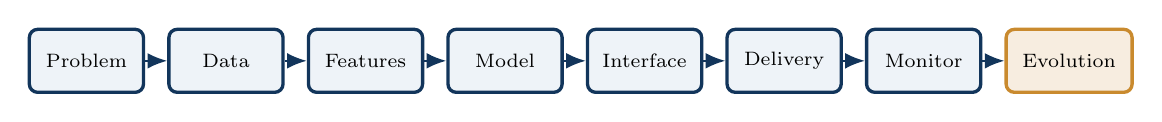
\begin{tikzpicture}[node distance=0.28cm]
  \node[flowbox, minimum width=1.45cm, minimum height=0.8cm] (problem) {\scriptsize Problem};
  \node[flowbox, minimum width=1.45cm, minimum height=0.8cm, right=of problem] (data) {\scriptsize Data};
  \node[flowbox, minimum width=1.45cm, minimum height=0.8cm, right=of data] (features) {\scriptsize Features};
  \node[flowbox, minimum width=1.45cm, minimum height=0.8cm, right=of features] (model) {\scriptsize Model};
  \node[flowbox, minimum width=1.45cm, minimum height=0.8cm, right=of model] (interface) {\scriptsize Interface};
  \node[flowbox, minimum width=1.45cm, minimum height=0.8cm, right=of interface] (delivery) {\scriptsize Delivery};
  \node[flowbox, minimum width=1.45cm, minimum height=0.8cm, right=of delivery] (monitor) {\scriptsize Monitor};
  \node[accentbox, minimum width=1.6cm, minimum height=0.8cm, right=of monitor] (evolution) {\scriptsize Evolution};
  \foreach \a/\b in {problem/data,data/features,features/model,model/interface,interface/delivery,delivery/monitor,monitor/evolution} {
    \draw[arrow] (\a) -- (\b);
  }
  \end{tikzpicture}

  \vspace{0.5em}
  \begin{block}{Today in the course}
  \textbf{Focus:} #1

  \textbf{Bridge:} #2
  \end{block}

  \begin{columns}[T]
  \column{0.48\textwidth}
  \begin{block}{Fraud case}
  {\footnotesize #3}
  \end{block}
  \column{0.48\textwidth}
  \begin{block}{Pasteurization case}
  {\footnotesize #4}
  \end{block}
  \end{columns}

  \vspace{0.3em}
  {\footnotesize \textbf{Course thread:} #5}
  \coursefooter
  \end{frame}
}

\newcommand{\classclosingframe}[4]{
  \begin{frame}{From This Class to the Next}
  \begin{block}{What stays with us}
  #1
  \end{block}

  \begin{columns}[T]
  \column{0.48\textwidth}
  \begin{block}{Project use}
  {\footnotesize #2}
  \end{block}
  \column{0.48\textwidth}
  \begin{block}{Next connection}
  {\footnotesize #3}
  \end{block}
  \end{columns}

  \vspace{0.3em}
  {\footnotesize \textbf{Course thread:} #4}
  \coursefooter
  \end{frame}
}

\tikzset{
  flowbox/.style={
    rounded corners=3pt,
    draw=courseblue,
    fill=courseice,
    very thick,
    minimum width=2.2cm,
    minimum height=0.9cm,
    align=center,
    font=\small
  },
  accentbox/.style={
    rounded corners=3pt,
    draw=coursegold,
    fill=coursegold!15,
    very thick,
    minimum width=2.2cm,
    minimum height=0.9cm,
    align=center,
    font=\small
  },
  arrow/.style={
    -{Latex[length=2.5mm,width=2mm]},
    thick,
    draw=courseblue
  }
}


\title{Class 6: Decision Support, APIs, and User Interfaces}
\author{\coursename}
\date{}

\begin{document}

\frame{\titlepage \coursefooter}

\begin{frame}{Agenda}
\begin{itemize}
\item From prediction to decision support.
\item Why model interfaces matter.
\item Flask as a service layer and Streamlit as a presentation layer.
\item Repository examples for fraud detection and streaming dashboards.
\item Risks: input validation, thresholds, logging, and trust.
\end{itemize}
\coursefooter
\end{frame}

\begin{frame}{Learning goals}
\learninggoals{
\begin{itemize}
\item Distinguish a prediction from a decision.
\item Explain the roles of APIs and dashboards in ML systems.
\item Compare Flask and Streamlit in the context of this course.
\item Identify the minimum quality requirements for a credible model interface.
\end{itemize}
}
\coursefooter
\end{frame}

\coursecontextframe
{Interfaces that turn model outputs into usable decisions.}
{This class connects modeling work to the first real system boundary: APIs, dashboards, and human-facing decision support.}
{In the fraud case, the model becomes a scoring endpoint that other services or analysts can call and interpret.}
{In the pasteurization case, the model becomes a streaming dashboard where sensor state, prediction, and alert behavior are visible together.}
{Once a model has an interface, software engineering concerns become unavoidable rather than optional.}

\begin{frame}{A model creates value only through an interface}
\begin{itemize}
\item A trained model that nobody can call or interpret has limited practical value.
\item Interfaces make predictions available to users, services, and operational workflows.
\item The interface also shapes trust: input checks, response format, and clarity matter.
\end{itemize}
\coursefooter
\end{frame}

\begin{frame}{Prediction is not the final decision}
\begin{itemize}
\item A fraud score suggests escalation, not guilt.
\item A medical risk score supports a clinician, not a replacement for judgment.
\item A drift alert suggests investigation, not automatic panic.
\end{itemize}
\begin{block}{Engineering implication}
Interfaces should communicate uncertainty, threshold logic, and next actions when possible.
\end{block}
\coursefooter
\end{frame}

\begin{frame}{Flask and Streamlit play different roles}
\begin{tabularx}{\textwidth}{>{\bfseries}l X}
Flask & Best when we need programmable endpoints over HTTP, such as `POST /predict` or a streaming route. \\
Streamlit & Best when we need a fast interactive UI for demos, dashboards, or exploratory interfaces. \\
Together & A common pattern is Flask for the backend service and Streamlit for the human-facing interface. \\
\end{tabularx}
\coursefooter
\end{frame}

\begin{frame}{Repository flow}
\centering
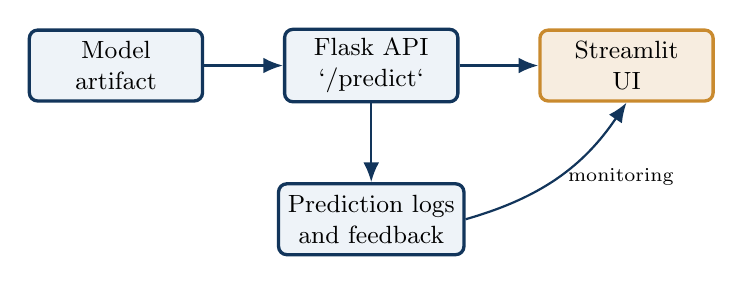
\begin{tikzpicture}[node distance=1cm and 1cm]
\node[flowbox] (model) {Model\\artifact};
\node[flowbox, right=of model] (api) {Flask API\\`/predict`};
\node[accentbox, right=of api] (ui) {Streamlit\\UI};
\node[flowbox, below=of api] (logs) {Prediction logs\\and feedback};
\draw[arrow] (model) -- (api);
\draw[arrow] (api) -- (ui);
\draw[arrow] (api) -- (logs);
\draw[arrow, bend right=20] (logs.east) to node[right, font=\scriptsize] {monitoring} (ui.south);
\end{tikzpicture}
\coursefooter
\end{frame}

\begin{frame}{Concrete repository examples}
\repoactivity{
\begin{itemize}
\item `Class6_model_api.py` exposes a basic prediction service through Flask.
\item `streamlit/pages/App_Credit_Card.py` turns a fraud model into an interactive decision-support interface.
\item `pasteurization/serving.py` exposes synthetic streaming sensor data through Flask.
\item `streamlit/pages/App_Pasteurization.py` and `App_Stream.py` consume live data for visualization and monitoring.
\end{itemize}
}
\coursefooter
\end{frame}

\begin{frame}[fragile]{Repository example: minimal Flask prediction endpoint}
\begin{lstlisting}[style=coursepython]
@app.route("/predict", methods=["POST"])
def predict():
    data = request.get_json(force=True)
    features = np.array(data["features"]).reshape(1, -1)
    pred = model.predict(features)[0]
    return jsonify({"prediction": int(pred)})
\end{lstlisting}
\begin{itemize}
\item This comes directly from `Class6_model_api.py`.
\item It is useful pedagogically because students can immediately see where input schema, validation, and logging are still missing.
\end{itemize}
\coursefooter
\end{frame}

\begin{frame}[fragile]{Repository example: Streamlit decision-support interaction}
\begin{lstlisting}[style=coursepython]
if st.button("Predict Fraud Risk"):
    prediction = model.predict(scaled)[0]
    probability = model.predict_proba(scaled)[0][1]

    if prediction == 1:
        st.error(f"Fraud Probability: {probability:.2%}")
    else:
        st.success(f"Fraud Probability: {probability:.2%}")
\end{lstlisting}
\begin{itemize}
\item This mirrors `streamlit/pages/App_Credit_Card.py`.
\item The key difference from Flask is audience: a human user needs labels, context, and actionable feedback rather than raw JSON.
\end{itemize}
\coursefooter
\end{frame}

\begin{frame}{What a better API should include}
\begin{itemize}
\item A clear input schema.
\item Error handling for malformed or incomplete requests.
\item Stable JSON output with prediction and confidence where appropriate.
\item Logging hooks for later monitoring and debugging.
\item Health or status endpoints for operational checks.
\end{itemize}
\coursefooter
\end{frame}

\begin{frame}{What a better dashboard should include}
\begin{itemize}
\item A visible explanation of what the model does and does not do.
\item Controls that reflect meaningful business inputs, not arbitrary technical internals.
\item Results that support action: alert, score, trend, or explanation.
\item Consistent links to data provenance, model version, or monitoring signals.
\end{itemize}
\coursefooter
\end{frame}

\begin{frame}[fragile]{Streaming interface example: live learning loop}
\begin{lstlisting}[style=coursepython]
response = requests.get(URL)
data = response.json()["current_weather"]
temp = data["temperature"]
wind = data["windspeed"]

y_pred = model.predict_one({"wind": wind})
model.learn_one({"wind": wind}, temp)
adwin.update(abs(temp - (y_pred or 0)))
\end{lstlisting}
\begin{itemize}
\item `streamlit/pages/App_Stream.py` shows that some interfaces are not single-request forms but continuous monitoring surfaces.
\item This also links directly to drift detection and operational dashboards later in the course.
\end{itemize}
\coursefooter
\end{frame}

\begin{frame}{Where trust breaks down}
\begin{itemize}
\item The interface hides uncertainty.
\item The inputs shown to users do not match training assumptions.
\item The API accepts bad requests silently.
\item The dashboard makes a model look authoritative when it is only a demo.
\end{itemize}
\coursefooter
\end{frame}

\begin{frame}{Technology links}
\readinglist{
\href{https://flask.palletsprojects.com/en/stable/}{Flask documentation};\ 
\href{https://flask.palletsprojects.com/en/stable/tutorial/}{Flask tutorial};\ 
\href{https://docs.streamlit.io/}{Streamlit documentation};\ 
\href{https://docs.streamlit.io/get-started}{Get started with Streamlit}.
}
\coursefooter
\end{frame}

\classclosingframe
{\begin{itemize}
\item Interfaces translate model behavior into decisions, workflows, and user trust.
\item Flask and Streamlit solve related but different problems in system design.
\item Serving requires validation, error handling, and clarity about uncertainty.
\end{itemize}}
{Students should now see how the same model can appear as an API for integration or as a dashboard for monitoring and decision support.}
{Class 7 broadens the view from single applications to software engineering foundations: quality, architecture, maintainability, and lifecycle discipline.}
{Once the service exists, the next question is whether it is engineered well enough to survive real use and future change.}

\begin{frame}{Papers and materials}
\readinglist{
\href{https://research.google/pubs/pub46555/}{Sculley et al., Hidden Technical Debt in Machine Learning Systems};\ 
\href{https://12factor.net/}{The Twelve-Factor App};\ 
\href{https://www.oreilly.com/library/view/designing-machine-learning/9781098107956/}{Designing Machine Learning Systems};\ 
\href{https://docs.streamlit.io/}{Streamlit docs and examples}.
}
\coursefooter
\end{frame}

\end{document}
